\section{Simulation Analysis}
\label{sec:simulation}

\subsection{Operating Point Analysis for t<0}

\par Table~\ref{tab:op_tb0} shows the simulated operating point results for the circuit
under analysis, when t<0.
\begin{table}[H]
  \centering
  \begin{tabular}{|l|r|}
    \hline    
    {\bf Name} & {\bf Value [A or V]} \\ \hline
    c[i] & 0.000000e+00\\ \hline
gib[i] & -2.26373e-04\\ \hline
r1[i] & 2.161226e-04\\ \hline
r2[i] & -2.26373e-04\\ \hline
r3[i] & -1.02499e-05\\ \hline
r4[i] & 1.194589e-03\\ \hline
r5[i] & -2.26373e-04\\ \hline
r6[i] & 9.784660e-04\\ \hline
r7[i] & 9.784660e-04\\ \hline
v(1) & 5.125627e+00\\ \hline
v(2) & 4.903891e+00\\ \hline
v(3) & 4.446215e+00\\ \hline
v(4) & -1.97572e+00\\ \hline
v(5) & 4.934963e+00\\ \hline
v(6) & 5.635816e+00\\ \hline
v(7) & -1.97572e+00\\ \hline
v(8) & -2.98275e+00\\ \hline

  \end{tabular}
  \caption{Operating point. A variable followed by [i] or [current] is of type {\em current}
    and expressed in Ampere; other variables are of type {\it voltage} and expressed in
    Volt.}
  \label{tab:op_tb0}
\end{table}

\subsection{Analysis for t>0 - Natural Solution}

\par Table~\ref{tab:op_vs0} shows the simulated operating point results for the circuit
under analysis,  when t>0.

\begin{table}[H]
  \centering
  \begin{tabular}{|l|r|}
    \hline    
    {\bf Name} & {\bf Value [A or V]} \\ \hline
    gib[i] & 6.327120e-18\\ \hline
r1[i] & -6.04063e-18\\ \hline
r2[i] & 6.327120e-18\\ \hline
r3[i] & 2.864858e-19\\ \hline
r4[i] & 1.289989e-18\\ \hline
r5[i] & -2.78376e-03\\ \hline
r6[i] & 1.301043e-18\\ \hline
r7[i] & 2.625374e-18\\ \hline
v(1) & 0.000000e+00\\ \hline
v(2) & 6.197538e-15\\ \hline
v(3) & 1.898958e-14\\ \hline
v(4) & -2.62707e-15\\ \hline
v(5) & 5.329071e-15\\ \hline
v(6) & 8.618561e+00\\ \hline
v(7) & -2.62707e-15\\ \hline
v(8) & -5.32907e-15\\ \hline

  \end{tabular}
  \caption{Operating point. A variable followed by [i] or [current] is of type {\em current}
    and expressed in Ampere; other variables are of type {\it voltage} and expressed in
    Volt.}
  \label{tab:op_vs0}
\end{table}

\begin{figure}[h] \centering
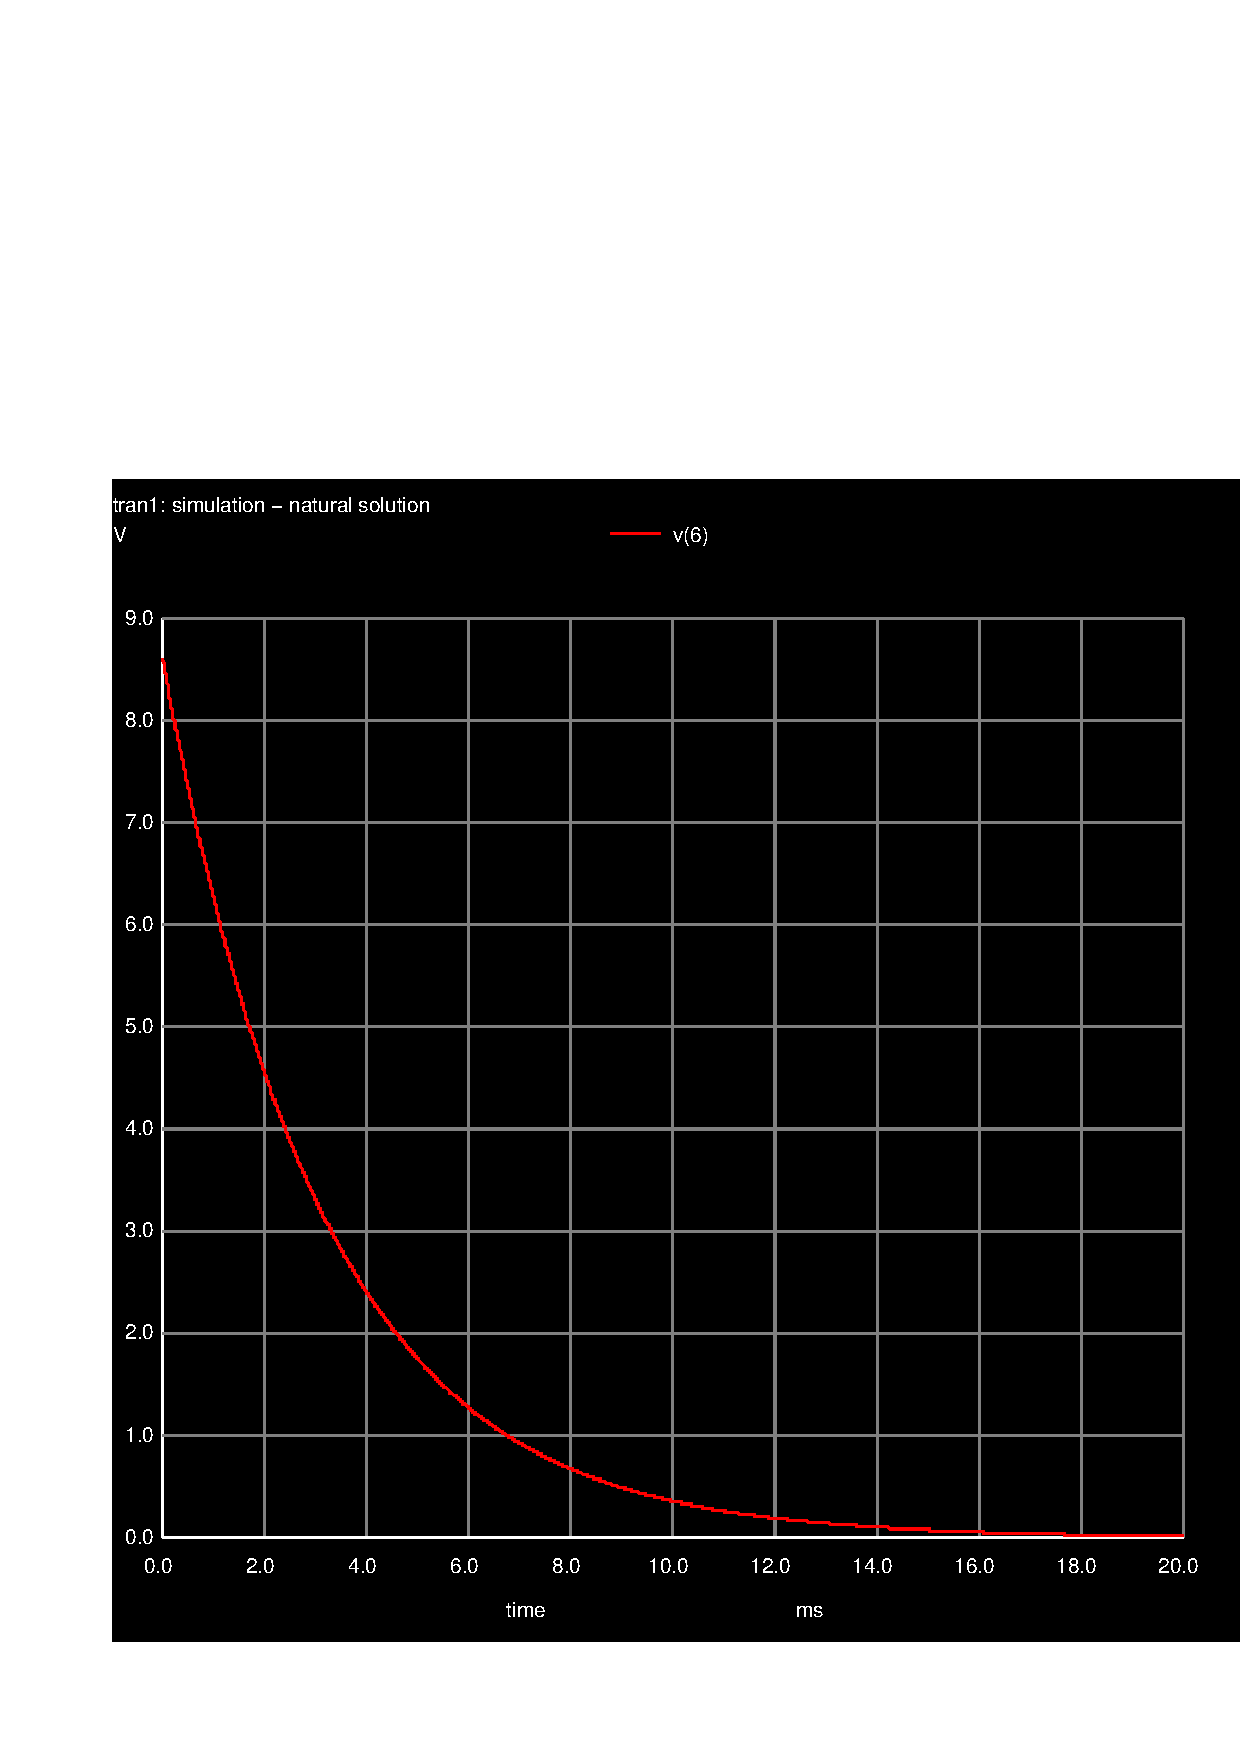
\includegraphics[width=0.6\linewidth]{trans_nat.pdf}
\caption{Natural solution}
\label{fig:trans_nat}
\end{figure}

\subsection{Analysis for t>0 - Total Solution}

\begin{figure}[h] \centering
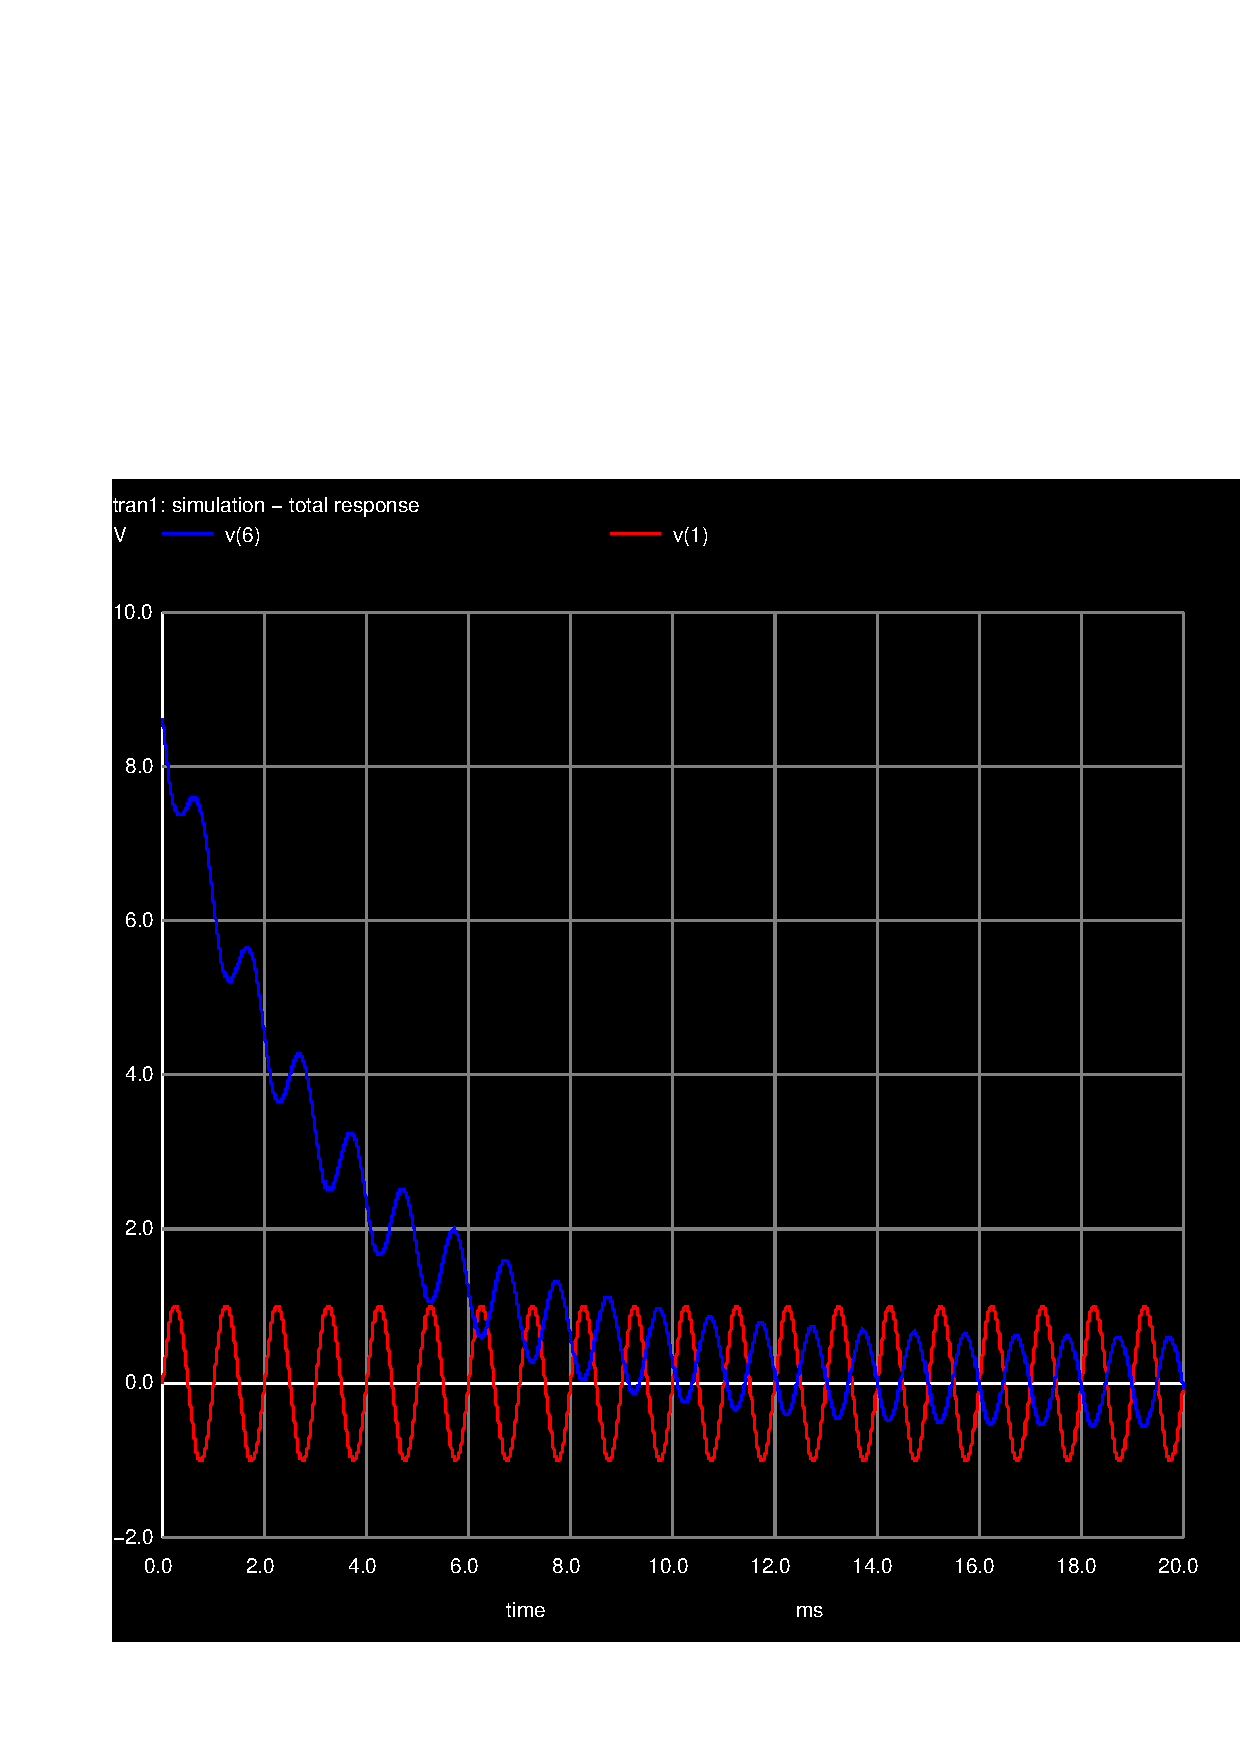
\includegraphics[width=0.6\linewidth]{trans_tot.pdf}
\caption{Total solution of the voltage source and the capacitor}
\label{fig:trans_tot}
\end{figure}

\subsection{Frequency Response}

\begin{figure}[h] \centering
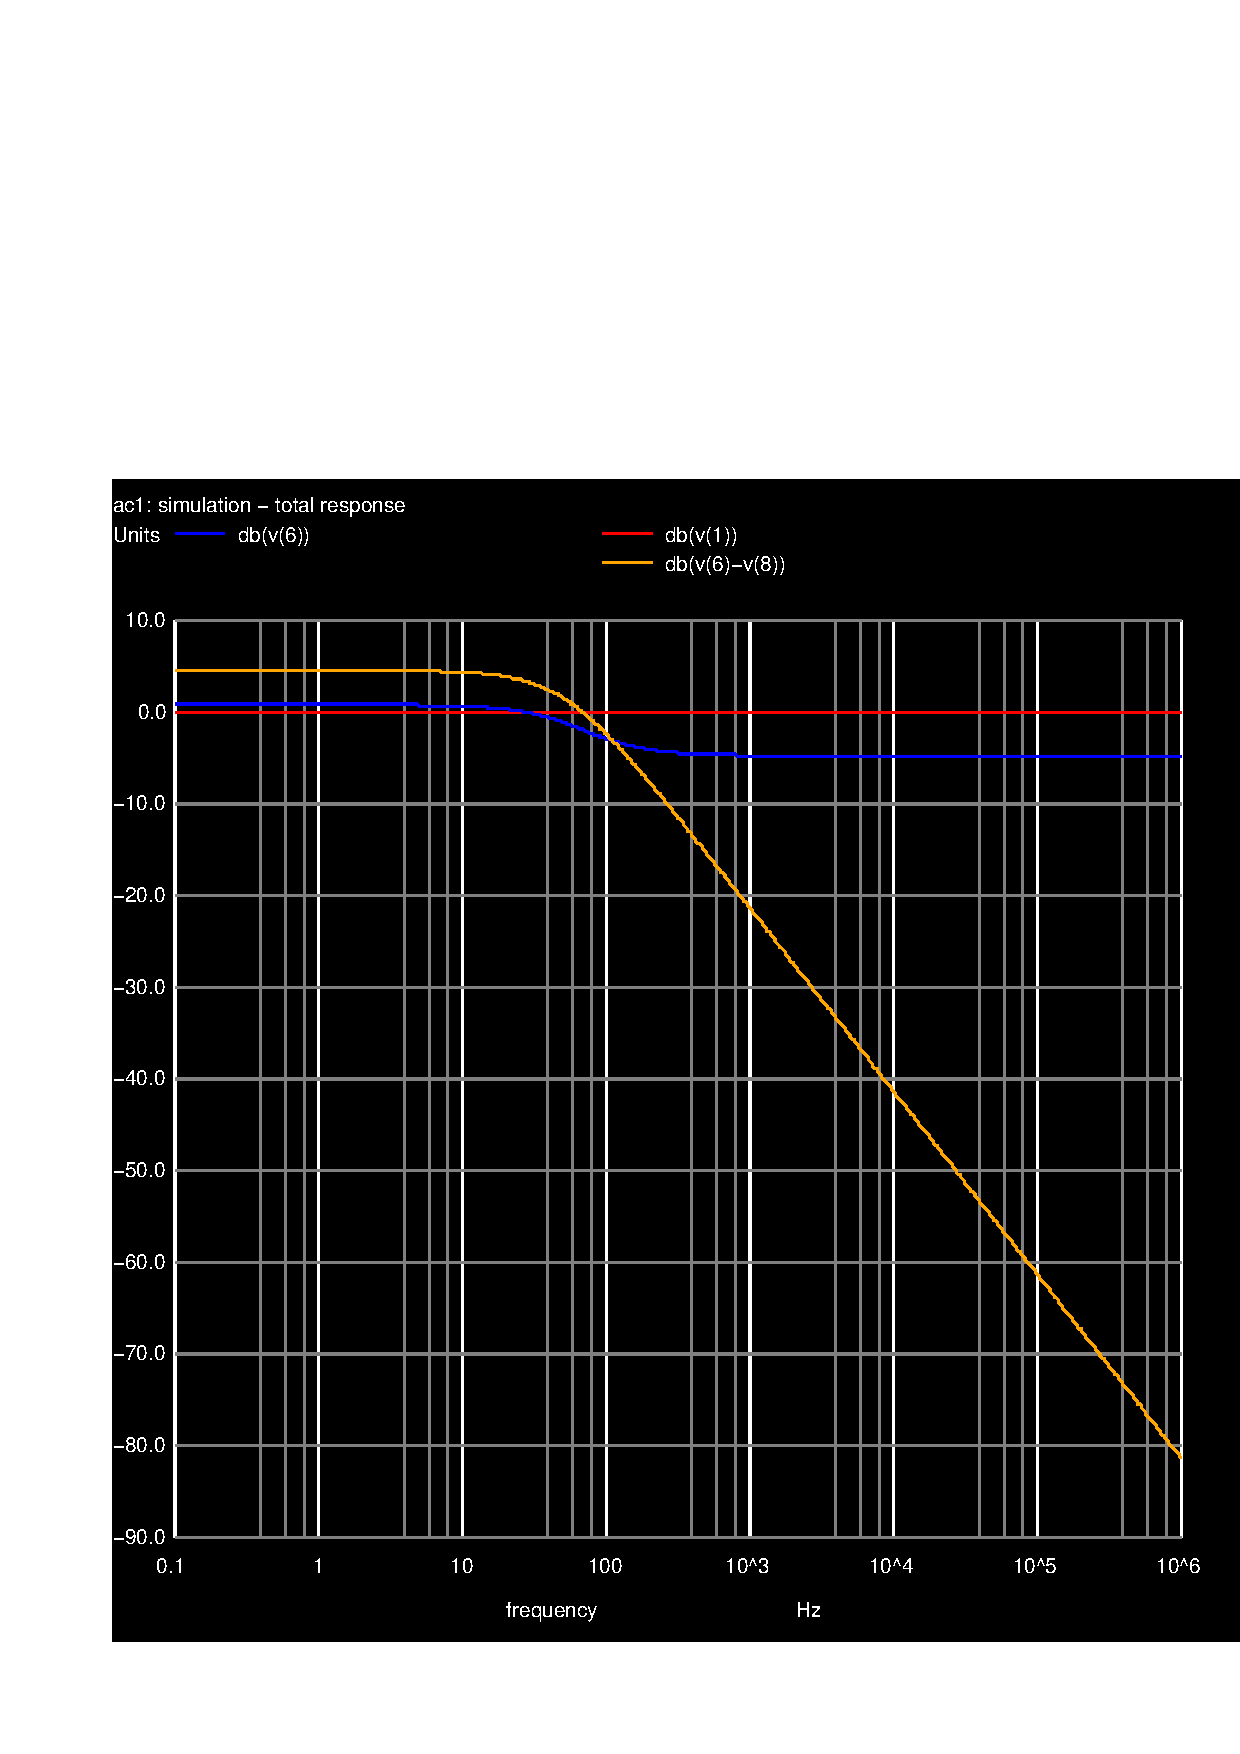
\includegraphics[width=0.6\linewidth]{db.pdf}
\caption{Magnitude in frequency response}
\label{fig:magnitude}
\end{figure}

\begin{figure}[h] \centering
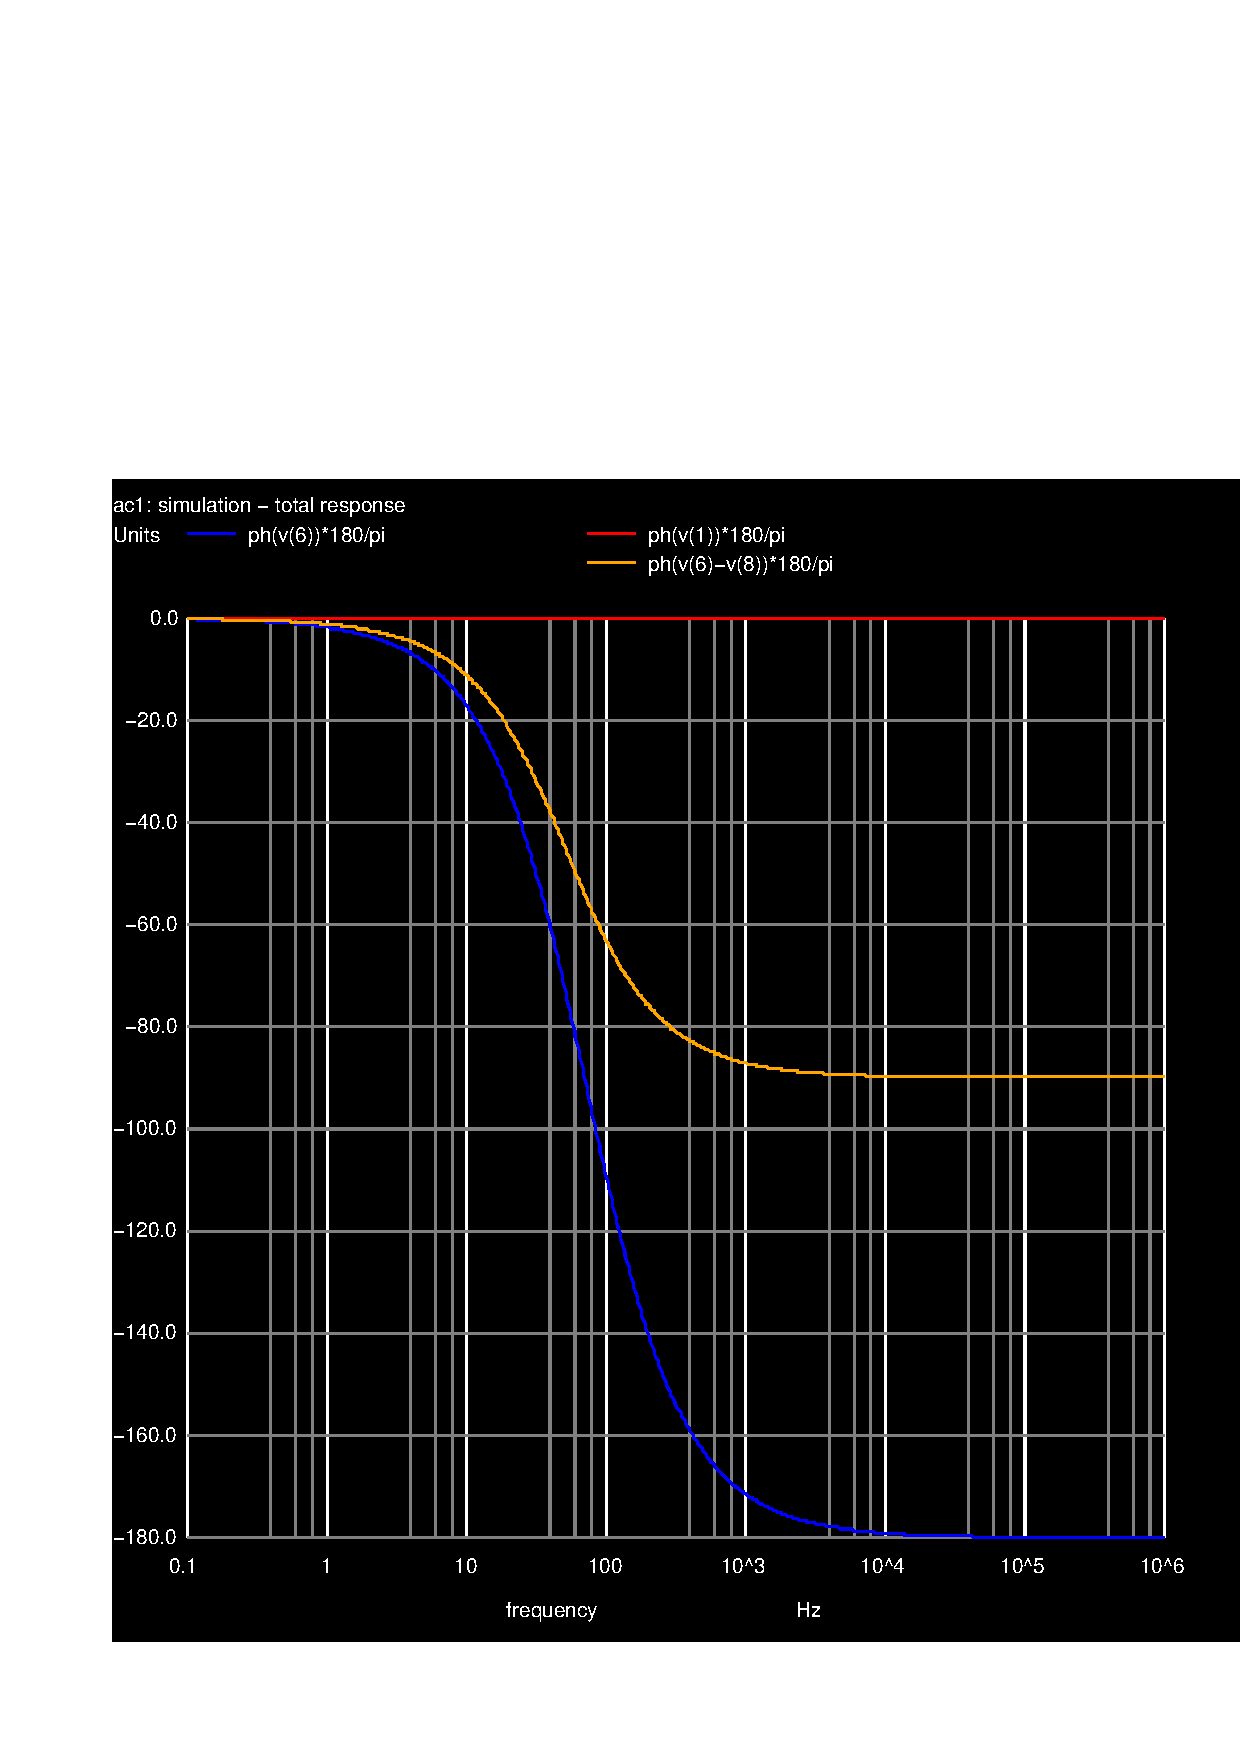
\includegraphics[width=0.6\linewidth]{ph.pdf}
\caption{Phase in frequency response}
\label{fig:phase}
\end{figure}











Table~\ref{tab:op} shows the simulated operating point results for the circuit
under analysis. Compared to the theoretical analysis results, one notices the
following differences: describe and explain the differences.

\begin{table}[h]
  \centering
  \begin{tabular}{|l|r|}
    \hline    
    {\bf Name} & {\bf Value [A or V]} \\ \hline
    I_b & -0.000226\\ \hline
I_d & 0.001012\\ \hline
I_{R1} & 0.000216\\ \hline
I_{R2} & -0.000226\\ \hline
I_{R3} & -0.000010\\ \hline
I_{R4} & 0.001195\\ \hline
I_{R5} & -0.001238\\ \hline
I_{R6} & 0.000978\\ \hline
I_{R7} & 0.000978\\ \hline
V_1 & 5.125627\\ \hline
V_2 & 4.903891\\ \hline
V_3 & 4.446215\\ \hline
V_4 & 8.768409\\ \hline
V_5 & -2.982745\\ \hline
V_6 & -1.975719\\ \hline
V_7 & 4.934963\\ \hline

  \end{tabular}
  \caption{Operating point. A variable preceded by @ is of type {\em current}
    and expressed in Ampere; other variables are of type {\it voltage} and expressed in
    Volt.}
  \label{tab:op}
\end{table}

\lipsum[1-1]


\subsection{Transient Analysis}

Figure~\ref{fig:trans} shows the simulated transient analysis results for the
circuit under analysis. Compared to the theoretical analysis results, one
notices the following differences: describe and explain the differences.

\begin{figure}[h] \centering
\includegraphics[width=0.6\linewidth]{trans.pdf}
\caption{Transient output voltage}
\label{fig:trans}
\end{figure}

\lipsum[1-1]



\subsection{Frequency Analysis}

\subsubsection{Magnitude Response}

Figure~\ref{fig:acm} shows the magnitude of the frequency response for the
circuit under analysis. Compared to the theoretical analysis results, one
notices the following differences: describe and explain the differences.

\begin{figure}[h] \centering
\includegraphics[width=0.6\linewidth]{acm.pdf}
\caption{Magnitude response}
\label{fig:acm}
\end{figure}

\lipsum[1-1]

\subsubsection{Phase Response}

Figure~\ref{fig:acp} shows the magnitude of the frequency response for the
circuit under analysis. Compared to the theoretical analysis results, one
notices the following differences: describe and explain the differences.

\begin{figure}[h] \centering
\includegraphics[width=0.6\linewidth]{acp.pdf}
\caption{Phase response}
\label{fig:acp}
\end{figure}

\lipsum[1-1]

\subsubsection{Input Impedance}

Figure~\ref{fig:zim} shows the magnitude of the frequency response for the
circuit under analysis. Compared to the theoretical analysis results, one
notices the following differences: describe and explain the differences.

\begin{figure}[h] \centering
\includegraphics[width=0.6\linewidth]{zim.pdf}
\caption{Input impedance}
\label{fig:zim}
\end{figure}

\lipsum[1-1]



